\section{SE-JEPA}
\label{sec:method}

\subsection{Motivation}
\label{sec:problem}
\label{sec:setting}
\label{sec:diagnosis}

Consider two episodes in which the agent pushes the same unfamiliar object toward different goals. The first may reveal how an off-center push rotates the object. That observation can help the agent choose a push in the second episode, even when it approaches the object from a different side. An episodic learner corrects its predictions along the first trajectory~\cite{wang2026adajepa}. Carrying its weights forward assumes that the next trajectory calls for a similar correction.

On a stream of PushObj goals, starting each episode from the preceding episode's final weights solved fewer goals than resetting the model (Appendix~D). Consecutive weight updates also point in nearly orthogonal directions (\supref{D}). A trajectory offers a different way to retain what the agent learned. Each executed action and its observed outcome provide a training example that can be revisited alongside contacts from later episodes.

\ours keeps a fast model for the current episode and trains a slow predictor on trajectories from multiple encounters (Fig.~\ref{fig:architecture}). The agent receives no labels telling it when a shape or appearance recurs. It groups trajectories by how they change the model and how well a common predictor explains them. When a new goal arrives, the first few actions provide evidence for which predictor to use.


\subsection{Fast adaptation and replay consolidation}
\label{sec:fast}
\label{sec:slow}

Each episode starts with working copies of the fixed pretrained encoder $E_0$ and predictor $P_0$. The planner minimizes latent goal cost over candidate action sequences~\cite{zhou2024dinowm,maes2026lewm} and executes the first action block. Following AdaJEPA~\cite{wang2026adajepa}, one Adam step on recent transition errors updates the predictor's last block and encoder head before replanning. These changes last only for the episode. Early replans can also retrieve a slow predictor as an \mbox{adaptation base (Sec.~\ref{sec:trust})}.

Across episodes, each \emph{predictive domain} $k$ maintains a replay buffer $\replay_k$ and slow predictor $P_{\phi_k}$. The frozen encoder re-encodes each accepted trajectory, keeping replay in a consistent latent space despite fast encoder changes. The slow predictor minimizes next-observation error on sampled replay windows:
\begin{equation}
  \loss_k(\phi_k)=
  \mathbb{E}_{(x,z^+)\sim\replay_k}
  \big\|P_{\phi_k}(x)-z^+\big\|_2^2.
  \label{eq:replay}
\end{equation}
Here $x$ contains observation embeddings and executed actions from a short history, and $z^+$ is the next observation embedding. Each slow predictor starts as a separate copy of $P_0$. Sampling windows across episodes combines different contacts and motions in the frozen representation space.

\subsection{Discovering predictive domains}
\label{sec:write}

The frozen reference first tests whether an episode contributes new experience. Let $\ell^{(0)}_{e,t}$ be its next-frame prediction error, and $\mathcal{I}_e$ index up to the first three observed transitions. Their geometric mean is
\begin{equation}
  F_e=\exp\!\left(\frac{1}{|\mathcal{I}_e|}
  \sum_{t\in\mathcal{I}_e}\log\ell^{(0)}_{e,t}\right).
  \label{eq:familiarity}
\end{equation}
If $F_e<\tau_f$, the calibrated familiarity threshold, the agent keeps $P_0$ as its adaptation base and skips the episode's direct memory write. Replay thus receives episodes the reference cannot yet predict accurately.

For an unfamiliar episode, $\Delta_e$ concatenates the fast predictor and encoder-head changes. Its normalized direction and similarity to domain $k$ are
\begin{equation}
  u_e=\frac{\Delta_e}{\|\Delta_e\|_2},
  \qquad s(e,k)=u_e^\top c_k,
  \label{eq:fingerprint}
\end{equation}
where $c_k$ is the domain's unit-length prototype. The retrieved domain is the first write candidate; otherwise, candidates are ranked by $s(e,k)$. The trajectory is assigned to a candidate domain if its predictor passes the error check in Sec.~\ref{sec:trust}. Unassigned trajectories remain in a pending pool. When a new direction aligns with those of two waiting episodes, the three trajectories establish a new domain.

Fingerprints propose candidates; prediction errors decide whether trajectories can share a learner. Delayed creation gathers evidence before fitting a new predictor. Domains merge when their predictors transfer in both directions: the larger domain retains its predictor, combines the buffers, and replays the merged experience. The frozen base remains available. Mature domains can also absorb smaller compatible groups (\supref{A}).

% Queue result displays for the next page, alongside the experiments.
% Declare experimental floats early so they accompany the results, before Conclusion.

\begin{table*}[!t]
  \centering
  \caption{\textbf{Goal-conditioned planning with CEM.} Zhou et al.~\cite{zhou2024dinowm} evaluate PushObj on two unseen shapes. Our PushObj evaluation covers seven shapes, including three unseen during pretraining. PushT covers six shifts, including three recolorings. Success is in percent. Steps is the mean replan count, with failures counted as 30. Rope and granular report Chamfer distance. Italics denote published results; bold compares the matched methods below the rule. $^{\mathrm{o}}$: offline PushT adapter; $^{\mathrm{T}}$: T-only checkpoint in our rigid-object runs.}
  \label{tab:main}
  \small
  \setlength{\tabcolsep}{3.5pt}
  \begin{tabular}{@{}lccccccccc@{}}
    \toprule
    & PushObj~\cite{zhou2024dinowm} & \multicolumn{3}{c}{PushObj (this study)} & \multicolumn{3}{c}{PushT visual shifts} & Rope & Granular\\
    \cmidrule(lr){2-2}\cmidrule(lr){3-5}\cmidrule(lr){6-8}\cmidrule(lr){9-9}\cmidrule(lr){10-10}
    Method & Unseen (2) $\uparrow$ & All (7) $\uparrow$ & Unseen (3) $\uparrow$ & Steps $\downarrow$
      & Shift (6) $\uparrow$ & Color (3) $\uparrow$ & Steps $\downarrow$ & CD $\downarrow$ & CD $\downarrow$\\
    \midrule
    \inputrows{tables/main_rows.tex}
    \bottomrule
  \end{tabular}
\end{table*}

\begin{figure*}[!t]
  \centering
  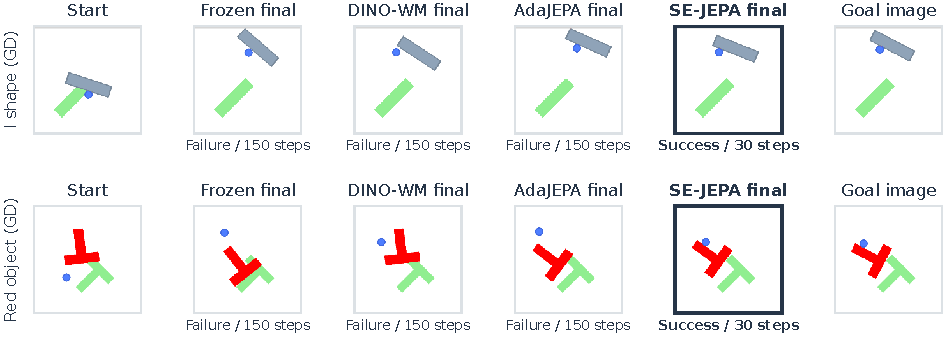
\includegraphics[width=\textwidth]{qualitative.pdf}
  \caption{\textbf{Persistent memory resolves failures of episodic adaptation.} Selected GD examples on an unseen I shape (top) and red-object shift (bottom). Frozen and AdaJEPA exhaust 30 replans in both cases; \textbf{\ours} succeeds in six and seven, respectively. Each row shares the same start and goal. The goal image specifies the pusher position and object pose; the green marker is static.}
  \label{fig:qualitative}
\end{figure*}

\begin{figure*}[!t]
  \centering
  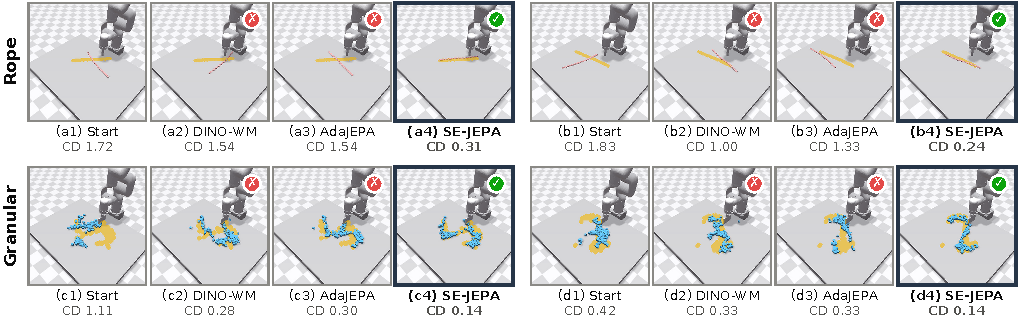
\includegraphics[width=\textwidth]{deform_qualitative.pdf}
  \caption{\textbf{Consolidated predictions support deformable manipulation.} Real FleX simulator trajectories for rope (top) and granular material (bottom), with two instances per task. Each group shows the start and the three methods' final states after 15 pushes; gold denotes the goal. These third-pass examples illustrate successful slow-only consolidation and were selected where both baselines fail. Frozen DINO-WM frames replay its executed actions. The aggregate fourth-pass results are reported in Table~\ref{tab:main}.}
  \label{fig:deform_qualitative}
\end{figure*}

\begin{figure}[!t]
  \centering
  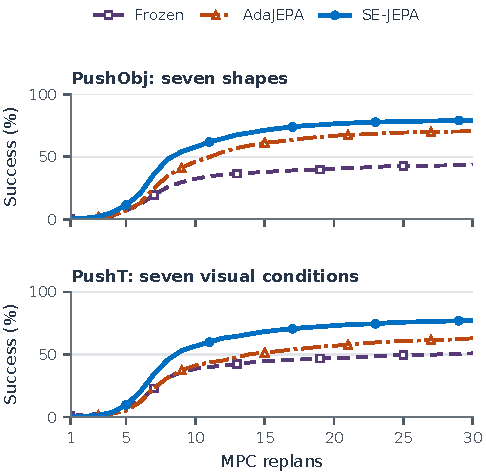
\includegraphics[width=\linewidth]{planning_efficiency.pdf}
  \caption{\textbf{Higher success within the same interaction budget.} Cumulative held-out success under CEM. Curves use all seven shapes (top) and all seven visual conditions (bottom).}
  \label{fig:efficiency_main}
\end{figure}

\begin{figure}[!t]
  \centering
  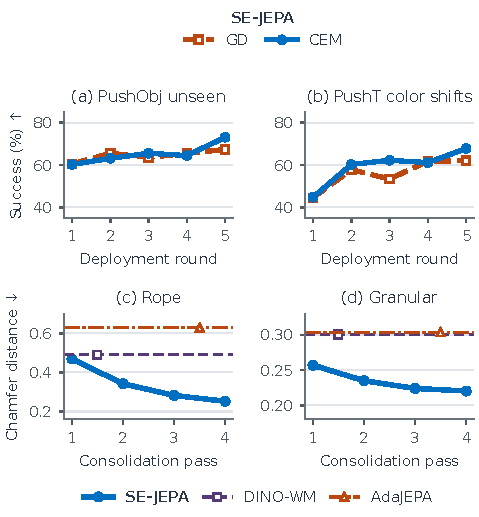
\includegraphics[width=\linewidth]{learning_progress.pdf}
  \caption{\textbf{Deployment experience improves two backbone families.} Top: ResNet-based models, with five rounds of online success on unseen PushObj shapes and three PushT color shifts; curves average three learning chains with targets resampled each round. Bottom: DINO-WM, with four consolidation passes over 50 fixed rope or granular instances; curves show mean CD. The horizontal lines are frozen DINO-WM and AdaJEPA.}
  \label{fig:deployment}
\end{figure}


\subsection{Validated retrieval for planning}
\label{sec:trust}

A slow predictor becomes eligible for planning by predicting new trajectories accurately before training on them. Before adding trajectory $\tau_e$ to a buffer, the agent rolls out the candidate predictor and the pretrained reference under the actions actually taken. Their open-loop errors in the frozen latent space give the ratio
\begin{equation}
  r_{e,k}=
  \frac{\loss_{\mathrm{roll}}(\phi_k;\tau_e)}
       {\loss_{\mathrm{roll}}(\theta_0;\tau_e)}.
  \label{eq:ratio}
\end{equation}
Here $\theta_0$ denotes the weights of $P_0$. Scoring both predictors on the same actions controls for trajectory difficulty. A write is rejected when $r_{e,k}>1.2$ in the rigid-object experiments. Accepted episodes record predictive transfer before replay training. A domain becomes eligible for retrieval when the arithmetic mean of its last three validation ratios is at most 0.9. Write acceptance admits useful experience, while the stricter maturity threshold requires consistent predictive improvement before the learner can guide planning.

During the first three replans, the agent compares eligible predictors and $P_0$ on the transitions observed so far, $\mathcal{B}_{e,t}$. It selects the predictor with the lowest recent error,
\begin{equation}
  k^\star=\argmin_{k\in\{0\}\cup\mathcal{K}_{\mathrm{eligible}}}
  \loss_{\mathrm{pred}}(\phi_k;\mathcal{B}_{e,t}),
  \qquad \phi_0=\theta_0.
  \label{eq:retrieval}
\end{equation}
The selected weights become the base of the fast predictor, preserving the corrections already made in the current episode. For an episode the reference recognizes as familiar, the base stays at $P_0$. Past trajectories therefore determine retrieval eligibility, while current observations determine which predictor guides planning.
